\section{Component Ablation Study}
\label{sec:ablation}

To dissect the specific contribution of each architectural component, we conduct an extensive ablation study on all 225 pairs of the SOICT-Data benchmark. Quantitative metrics are summarized in Table~\ref{tab:ablation_study}, and qualitative visualizations across components and prompt conditioning levels are presented in Figure~\ref{fig:ablation_components} and Figure~\ref{fig:ablation_prompts}.

% ==============================================================================
% Table 2: Component Ablation Study (Compact 8-column format without checkmarks)
% ==============================================================================
\begin{table*}[t]
\centering
\caption{\textbf{Ablation study on architectural components and hyperparameters of \method.} All metrics are scaled by $\times 100$. Evaluated on full 225 content-style pairs under null prompting. Removing either Score-Orthogonal Guidance (D) or AdaIN Pushforward (E) severely degrades structural fidelity ($\text{CLIP-I} \downarrow$, $\text{LPIPS} \uparrow$, $\text{DCL} \uparrow$).}
\label{tab:ablation_study}
\small
\begin{tabular}{lccccccc}
\toprule
\textbf{Configuration} & $\alpha_s$ & $\tau$ & \textbf{CSD} $\uparrow$ & \textbf{DINO} $\uparrow$ & \textbf{CLIP-I} $\uparrow$ & \textbf{LPIPS} $\downarrow$ & \textbf{DCL} $\downarrow$ \\
\midrule
\textbf{(A) Full \method} & 0.85 & 1 & 39.49 & 23.86 & \textbf{79.87} & \textbf{56.22} & \textbf{26.41} \\
(B) Pure Mean Token & 0.00 & 1 & 23.35 & 17.56 & 85.15 & 55.04 & 20.58 \\
(C) Raw Style Token & 1.00 & 1 & 52.64 & 34.38 & 68.94 & 67.92 & 44.82 \\
(D) w/o Score-Orthogonal Guidance & 0.85 & 1 & 46.66 & 30.96 & 70.80 & 70.19 & 43.26 \\
(E) w/o AdaIN Pushforward & 0.85 & 1 & 65.87 & 49.53 & 58.74 & 74.89 & 64.74 \\
(F) w/o Semantic Gated Canny & 0.85 & 1 & 44.98 & 30.36 & 71.13 & 69.88 & 42.23 \\
\midrule
\multicolumn{8}{l}{\textit{Pushforward Step Threshold Sweeps ($\tau \in \{1, 2, 3, 4\}$):}} \\
Sweep $\tau = 1$ & 0.85 & 1 & 45.14 & 27.34 & 75.90 & 58.55 & 27.27 \\
Sweep $\tau = 2$ & 0.85 & 2 & 41.57 & 25.51 & 76.50 & 56.61 & 25.50 \\
Sweep $\tau = 3$ & 0.85 & 3 & 40.40 & 24.54 & 78.44 & 55.51 & 23.52 \\
Sweep $\tau = 4$ & 0.85 & 4 & 37.07 & 23.27 & 79.40 & 54.22 & 21.65 \\
\midrule
\multicolumn{8}{l}{\textit{Prompt Conditioning Levels:}} \\
Prompt: Object Level (\texttt{"a <obj>"}) & 0.85 & 1 & 29.10 & 18.92 & 83.82 & 55.23 & 21.57 \\
Prompt: Style Level (\texttt{"<obj> in <sty>"}) & 0.85 & 1 & 40.23 & 25.21 & 78.01 & 59.98 & 30.00 \\
\bottomrule
\end{tabular}
\end{table*}

\paragraph{Analysis of Component Contributions.}
\begin{enumerate}
    \item \textbf{Impact of Blended Style Tokens ($\alpha_s$)}: Setting $\alpha_s = 0.0$ (Configuration B, pure mean pooling as in RB-Modulation) degrades texture fidelity, causing CSD to collapse from $39.49$ to $23.35$ and DINO from $23.86$ to $17.56$. Conversely, using raw, unblended style tokens ($\alpha_s = 1.0$, Configuration C) allows foreign style semantics to intrude, dropping CLIP-I from $79.87$ to $68.94$ and elevating leakage DCL to $44.82$. The blended parameter $\alpha_s = 0.85$ achieves the optimal trade-off, transferring rich texture while filtering semantic noise.
    \item \textbf{Necessity of Score-Orthogonal Guidance}: When orthogonal projection is disabled (Configuration D, standard gradient guidance), unconstrained gradients push latents off the data manifold, distorting content boundaries ($\text{CLIP-I}$ drops to $70.80$, $\text{LPIPS}$ degrades to $70.19$, and $\text{DCL}$ spikes to $43.26$). Projecting gradients strictly onto the null space of the score vector $\mathbf{s}_\theta$ eliminates this geometric corruption.
    \item \textbf{Role of Clean Latent AdaIN Pushforward}: Completely omitting the pushforward mechanism (Configuration E) causes catastrophic instability during initial diffusion steps: CLIP-I collapses to $58.74$, LPIPS escalates to $74.89$, and DCL worsens to $64.74$. Applying AdaIN on the predicted clean latent $\bx_0$ in early steps anchors global color and texture statistics, providing a stable foundation for subsequent denoising.
    \item \textbf{Efficacy of Semantic Gated Canny}: Removing background gating (Configuration F, standard Canny edge detection) captures noisy background contours, reducing generative freedom and degrading CLIP-I to $71.13$.
    \item \textbf{Controllability via Parameter $\tau$}: As shown in the sweep over $\tau \in \{1, 2, 3, 4\}$, increasing $\tau$ monotonically boosts content preservation ($\text{CLIP-I}$ increases from $75.90$ to $79.40$, while $\text{DCL}$ drops from $27.27$ to $21.65$). Users can thus smoothly navigate the Pareto frontier by selecting $\tau$ without retraining the network.
\end{enumerate}

% ==============================================================================
% Figure: Qualitative Ablation of Architectural Components
% ==============================================================================
\begin{figure*}[t]
\centering
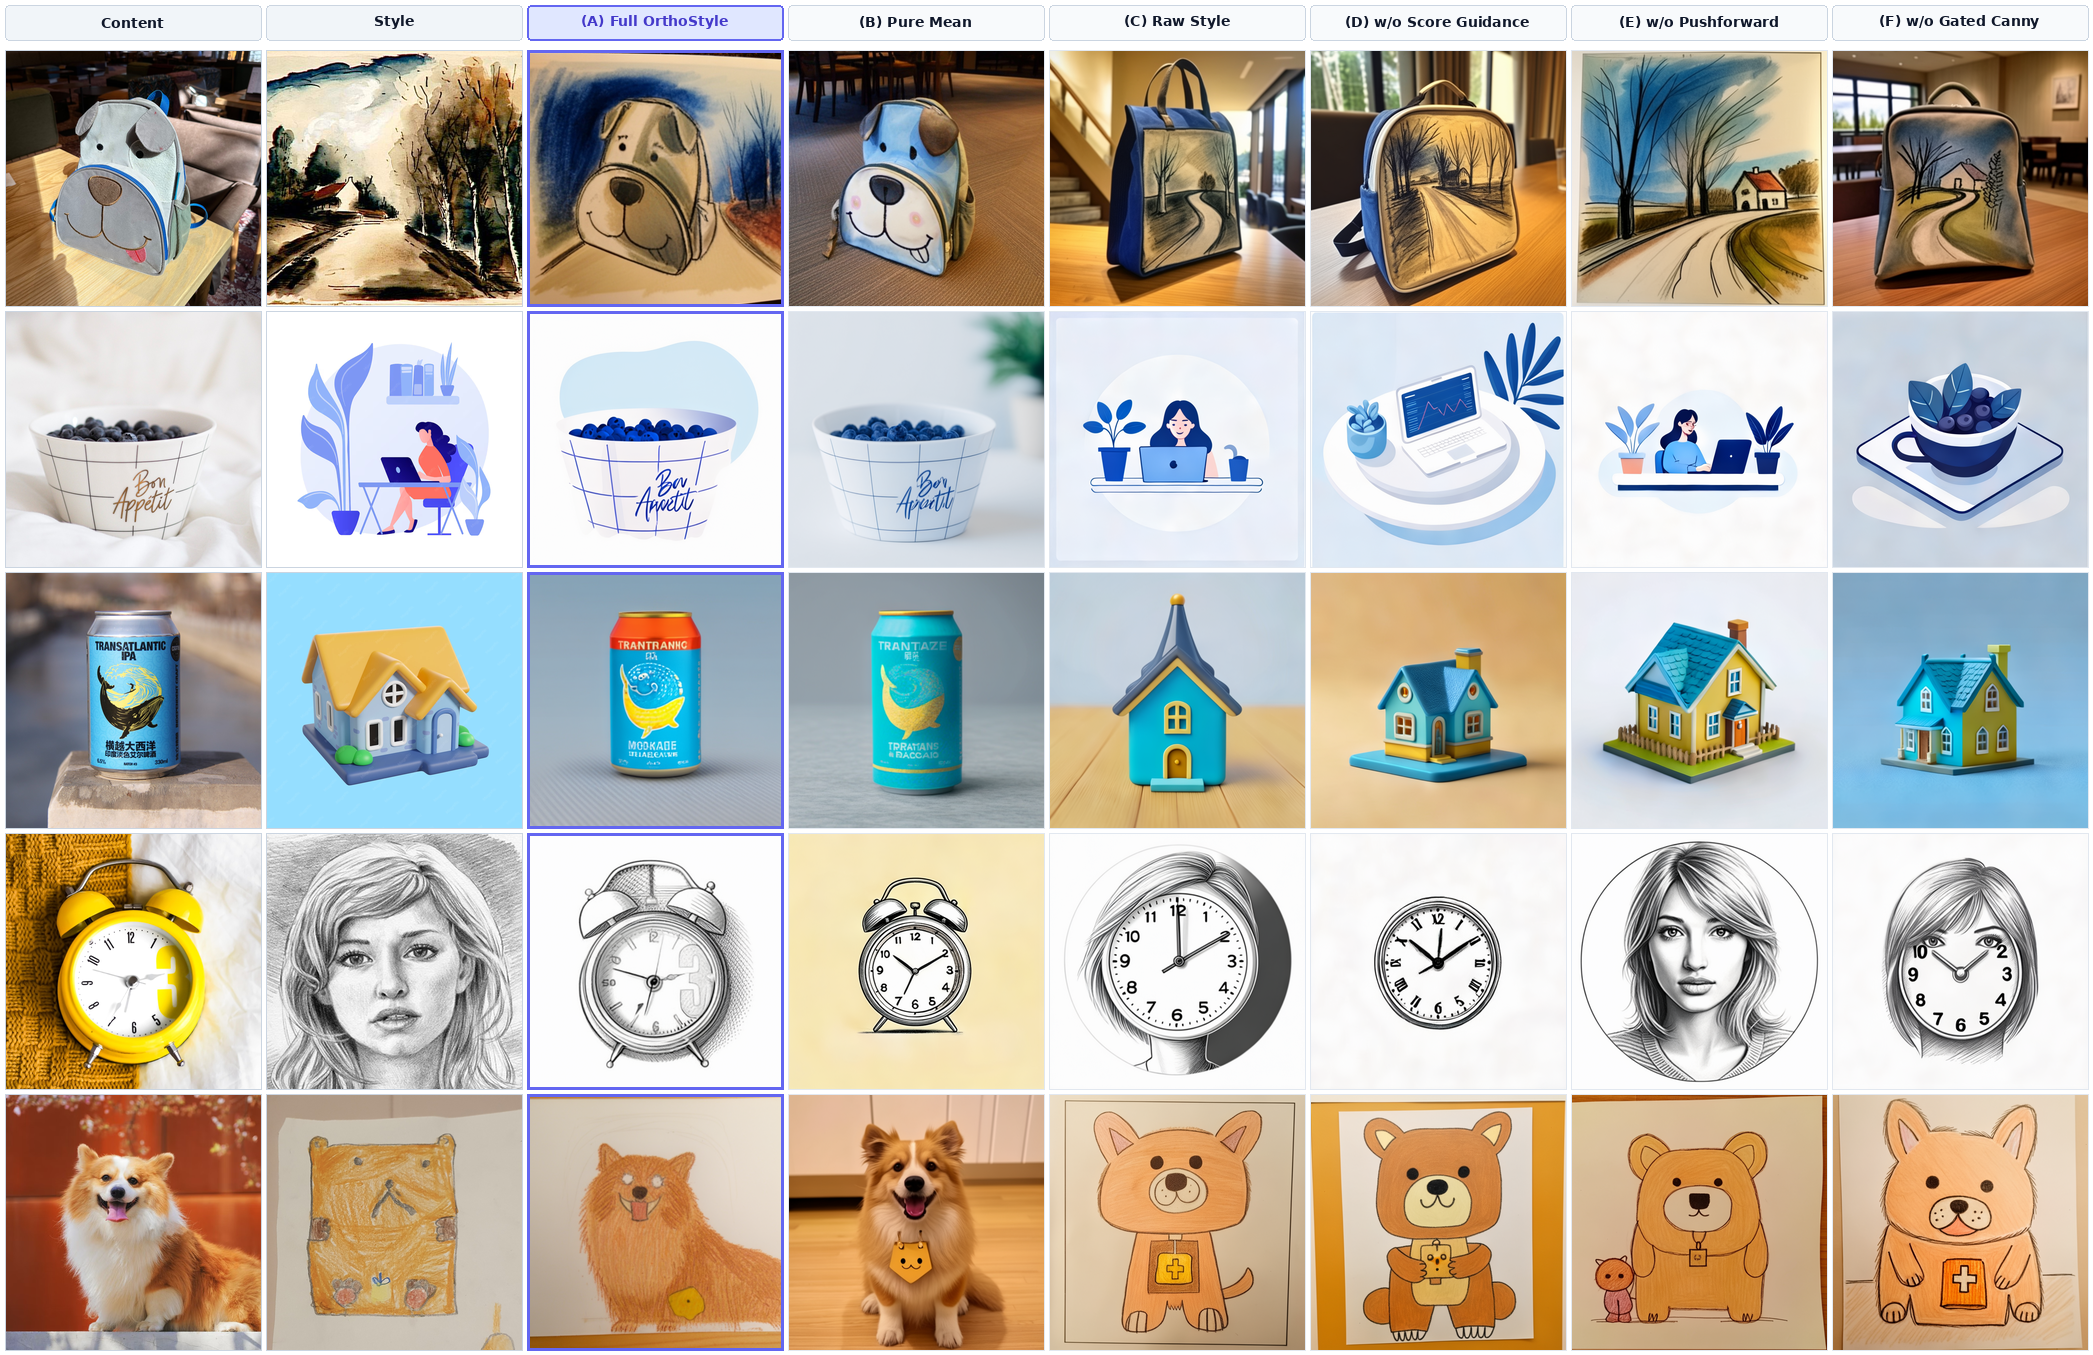
\includegraphics[width=\textwidth]{figs/ablation_components.png}
\caption{\textbf{Qualitative ablation of architectural components across diverse content-style matching pairs.} (A) Full \method provides balanced texture synthesis and silhouette preservation; (B) Pure mean pooling fails to transfer rich artistic stroke textures; (C) Raw style tokens allow foreign style objects to bleed into the subject; (D) Omitting score guidance degrades artistic vibrancy; (E) Removing early-step AdaIN pushforward severely disrupts global color distribution; (F) Disabling semantic edge gating introduces rigid background artifacts.}
\label{fig:ablation_components}
\end{figure*}

% ==============================================================================
% Figure: Qualitative Ablation across Prompt Conditioning Levels
% ==============================================================================
\begin{figure*}[t]
\centering
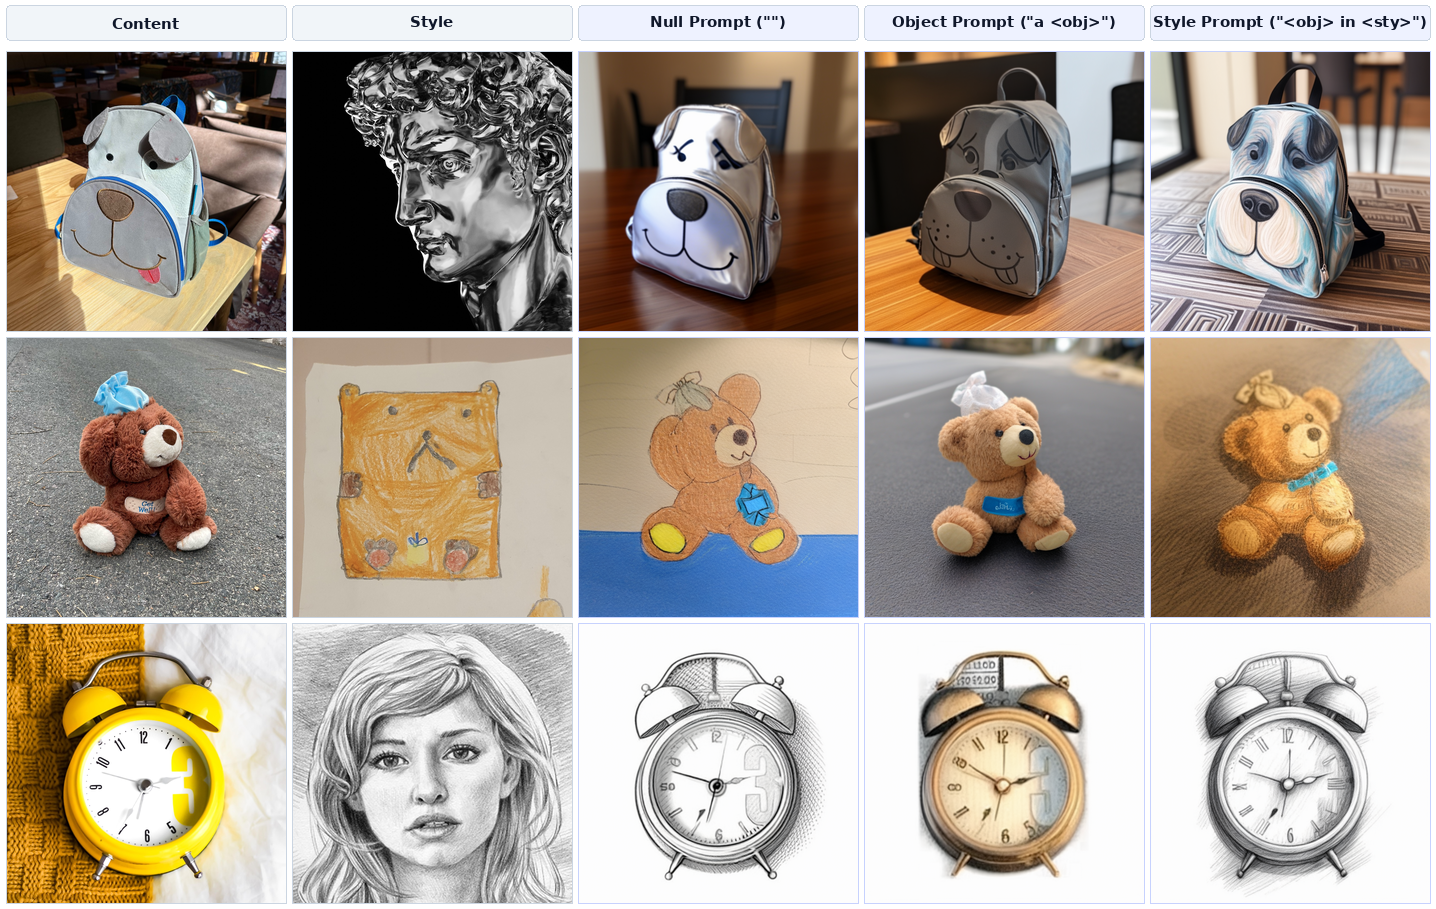
\includegraphics[width=0.95\textwidth]{figs/ablation_prompt_levels.png}
\caption{\textbf{Qualitative comparison across prompt conditioning levels.} Level 1 (Null prompt, \texttt{""}) relies purely on exemplar conditioning; Level 2 (Object prompt, \texttt{"a <obj>"}) reinforces target subject priors; Level 3 (Style prompt, \texttt{"<obj> in <sty> style"}) guides both subject identity and explicit artistic style keywords.}
\label{fig:ablation_prompts}
\end{figure*}
